\chapter{Gestión dinámica de la plataforma \textsc{alma}} 
\label{chapter:gestion-dinamica}

\begin{center}
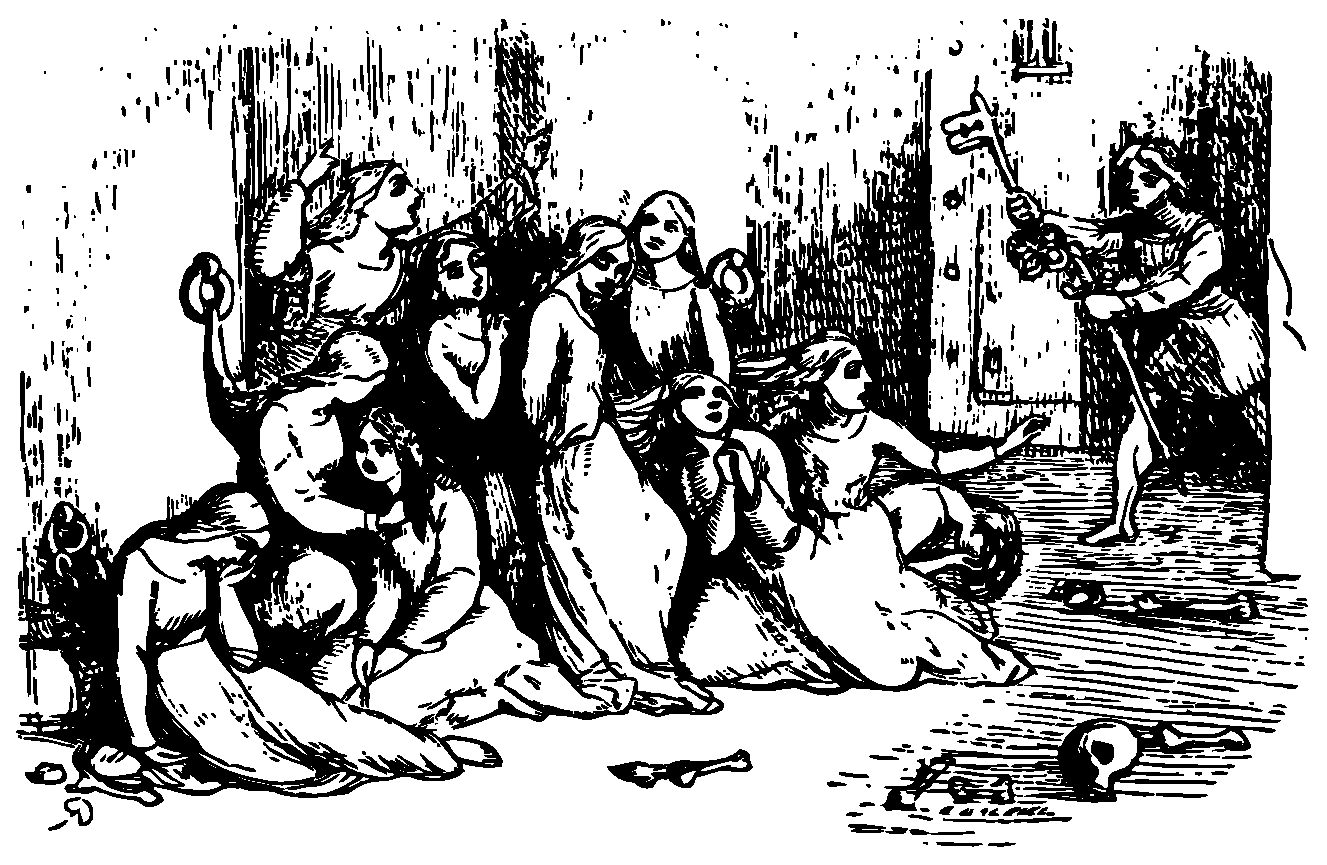
\includegraphics[scale=0.4]{../graphics/johnny_automatic_Jack_freeth_the_captives.eps}
\end{center}

\lettrine{E}{n este capítulo}, dividido en dos partes fundamentales, se mostrará en la primera que mejoras se han producido utilizando los \profiles{} (y desde el punto de vista de un administrador) en la creación de nuevas comunidades de práctica. En la segunda parte se mostrarán detalles internos de los \profiles{} realizados (no obstante, para analizar las implementaciones completas de dichos \profiles{} se deberá visitar el \appendixref{apendice-b}, ya que, en este capítulo sólo se enseñarán los fragmentos que se consideran relevantes).

\section{¿Qué ha cambiado en la gestión de \tiki{} utilizando Profiles?}

\subsection{¿Cómo se crea una nueva asignatura?}

En esta nueva situación, crear asignaturas (comunidades de práctica) se ha convertido en una tarea muy simple (cuando antes no lo era). Los pasos que tiene que seguir el administrador o docente para crear una nueva asignatura son los siguientes (se asume que ya están instalados los \profiles{} diseñados para \alma{} correctamente, en el \appendixref{apendice-c} se encuentra el manual de usuario que explica como hacerlo de manera muy detallada):

\begin{enumerate}
\item El administrador o docente ha de listar todas las páginas \textit{wiki} que están disponibles en \tiki{} (\figureref{listar_paginas_wiki_profiles}). Ha de buscar una llamada: \texttt{Crear\_Comunidad\_de\_Practica\_GUI}, en ella se encuentra la interfaz por la cuál se puede ejecutar el \profile{} que se encuentra definido en otra página \textit{wiki} denominada: \texttt{Crear\_Comunidad\_de\_Practica\_Template}.

\begin{figure}
\centering
\includegraphics{../graphics/fig_listar_paginas_wiki_profiles.png}
\caption{Dado que el \profile{} es una página \textit{wiki} hay que buscar donde se encuentra éste.}\label{fig:listar_paginas_wiki_profiles}
\end{figure}

\item Una vez en la página \texttt{Crear\_Comunidad\_de\_Practica\_GUI} se escribe el nombre de la asignatura que se desee crear (\figureref{crear_asignatura_matematicas_profile}).

\begin{figure}
\centering
\includegraphics[width=\linewidth]{../graphics/fig_crear_asignatura_matematicas_profile.png}
\caption{Es tan sencillo como poner el nombre de la asignatura a crear y darle a Ir. El \profile{} se encargará del resto.}\label{fig:crear_asignatura_matematicas_profile}
\end{figure}

\item ¡Y listo, comunidad de práctica creada! A partir de ahora el administrador o docente deberá ir a la sección de usuarios y decidir quién quiere que sea miembro de dicha comunidad (\figureref{ejemplo_admin_usuarios}).
\end{enumerate}

\begin{figure}
\centering
\includegraphics[width=\linewidth]{../graphics/fig_ejemplo_admin_usuarios.png}
\caption{En el panel de usuarios se pueden agregar qué usuarios pertenecen a qué grupos. Por defecto, por cada comunidad de práctica que se crea, el usuario \textit{admin} pertenece a cada grupo de dicha comunidad.}\label{fig:ejemplo_admin_usuarios}
\end{figure}

\section{Implementación interna de los \profiles{} desarrollados}

\subsection{Profile que configura \tiki{} a las necesidades de \alma{}}

\subsubsection{Objetivo}

El objetivo principal de este \profile{} es configurar una nueva instalación de \tiki{} y modificarla a las necesidades del proyecto \alma{}. Esto presenta múltiples ventajas, entre ellas: 

\begin{itemize}
\item Nos permite replicar \alma{} de una manera muy rápida y cómoda para un administrador. Si, por ejemplo, la instalación que existe actualmente sobre \tiki{} desapareciese (por el motivo que fuere), se podría descargar de nuevo el programa, ejecutar dicho \profile{} y tener una réplica exacta de la anterior \alma{} en ajustes y preferencias. De esta manera el administrador de la plataforma sólo se tiene que preocupar por recuperar los datos que se hayan guardado en la anterior instalación e importarlos en la nueva. 

\item Como punto que parte del anterior, nos sirve también para crear una réplica de \alma{} para hacer nuestras pruebas internas sin afectar al servidor principal, es decir, como plataforma de desarrollo. Este es el método que ha usado el autor del \pfc{} para crear los demás \profiles{}.
\end{itemize}

\subsubsection{¿Cómo se ha implementado?}

La lógica que se ha utilizado para crear este \profile{} es la que sigue en la \figureref{configuracion_alma_profile}. A continuación, se explican las etapas una a una:

\begin{figure}
\centering
\includegraphics[width=\linewidth]{../graphics/fig_configuracion_alma_profile.eps}
\caption{Etapas empleadas para elaborar el \profile{} que configura \tiki{} a las necesidades de \alma{}.}\label{fig:configuracion_alma_profile}
\end{figure}

\begin{itemize}
\item \textit{Activación y desactivación de recursos}: Dado que \alma{} tiene unas necesidades muy concretas se han habilitado todos los elementos que hacen posible que funcionen las comunidades de práctica (entre ellos se activan los \profiles{}, las categorías y las perspectivas):

\begin{pyglist}[language=text]
  feature_categories:  y
  feature_mytiki: y
  feature_userPreferences: y
  feature_profiles: y
  feature_perspective: y
\end{pyglist}

Así mismo se desactivan múltiples características de \tiki{} que, en principio, no se van a utilizar (al menos por ahora). Si analizamos el \profile{}, encontraremos que se anulan los siguientes elementos: 

\begin{pyglist}[language=text]
  feature_blogs:  n  
  feature_file_galleries:  n
  feature_forums:  n
  feature_freetags:  n
  feature_help:  n
  feature_trackers: n
\end{pyglist}

\item \textit{Configuración del correo electrónico}: Se dan los datos necesarios para que se puedan enviar correos electrónicos desde la propia plataforma, ya sea para notificar a los usuarios de que se han registrado en una comunidad de práctica así como para recibir la contraseña en caso de extravío.

\begin{pyglist}[language=text]
  sender_email: alma@uah.es
  zend_mail_handler: smtp
  default_mail_charset: utf-8
  zend_mail_smtp_user: alma.disciplinar@gmail.com
  zend_mail_smtp_pass: password
  zend_mail_smtp_port: 465
  zend_mail_smtp_security: ssl
  zend_mail_smtp_auth: plain
  zend_mail_smtp_server: smtp.gmail.com
\end{pyglist}

\item \textit{Cambio del logotipo}: Se personaliza la imagen de \tiki{} sustituyendo el logotipo que trae por defecto a uno diseñado específicamente para \alma{}.

\begin{pyglist}[language=text]
  sitelogo_title: ALMA (Aula Libre Multidisciplinar Abierta)
  sitelogo_src: img/tiki/tikisitelogo.png
  sitelogo_alt: Alma
\end{pyglist}


\item \textit{Creación automática de los demás \profiles{}}: Por último se encarga de crear un grupo denominado \texttt{Profiles} donde se almacenarán los dos \profiles{} que se utilizan para crear comunidades de práctica (el \profile{} en si y su \textit{Data Channel} asociado).

\begin{pyglist}[language=text]
  objects:
    -
      type: wiki_page
      ref: wiki1
      data:
        name: Crear_Comunidad_de_Practica_GUI
        content: "{DATACHANNEL(channel=crear_comunidad)}
        nombre_asignatura, Nombre de la comunidad de practica
        {DATACHANNEL}"
    -
      type: wiki_page
      ref: wiki2
      data:
        name: Crear_Comunidad_de_Practica_Template
    -
      type: category
      ref: profilecateg
      data:
        name: Profiles
        items:
         - [ wiki_page, $wiki1 ]
         - [ wiki_page, $wiki2 ]
\end{pyglist}

Y se le asignan permisos específicos para que sólo los administradores puedan ver, editar y borrar todos los elementos que contenga dicha categoría.

\begin{pyglist}[language=text]
  permissions:
   Admins:
    objects:
     -
      type: category
      id: $profilecateg
      allow:
        - admin
\end{pyglist}

También se realizan los ajustes pertinentes (que no puedan ver, ni editar, ni borrar) para los demás grupos (\texttt{Registered}, \texttt{Anonymous}).

\begin{pyglist}[language=text]
   Registered:
    objects:
     -
      type: category
      id: $profilecateg
      deny: view, edit, view_category, edit_category
\end{pyglist}

\item \textit{Miscelánea}: Otros cambios que se realizan son las mejoras en los editores \wysiwyg{} (se añade la posibilidad de que los usuarios puedan crear fórmulas matemáticas) o se pone el lenguaje de \tiki{} en castellano.
 
 \begin{pyglist}[language=text]  
  language: es
  feature_wysiwyg:  y
  wysiwyg_default: y
  wysiwyg_optional: y
  wikiplugin_equation: y
  wikiplugininline_equation: y
\end{pyglist}

\end{itemize}

Si queremos analizar la implementación completa hay que visitar la \sectionnopageref{configuracion_alma} del \appendixref{apendice-b}.

\subsection{Profile que crea de manera automática comunidades de práctica} 

\subsubsection{Objetivo}

El objetivo de este conjunto de \profiles{} (se necesitan dos para llevar a cabo la tarea, aunque, el grueso de la operación realmente se produce en uno y el otro sirve como apoyo) está bastante claro. Por definición expresa, es el que simplifica la gestión de \tiki{} y son los que dan sentido completo a este \pfc{}.

\subsubsection{¿Cómo se ha implementado?}

Anteriormente se explicó como un administrador o docente podía crear una asignatura visitando la página \textit{wiki}: \texttt{Crear\_Comunidad\_de\_Practica\_GUI}. En la \figureref{esquema_flujo_profiles_interno} podemos ver como es realmente el flujo por detrás (la implementación que existe).

\begin{figure}
\centering
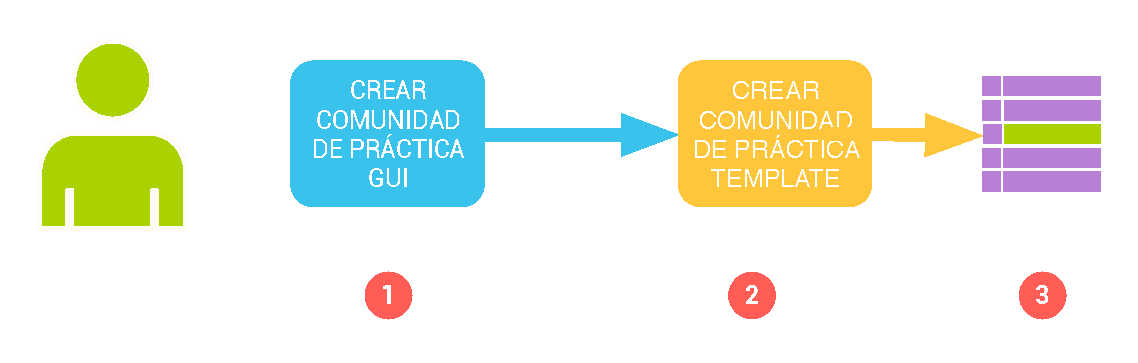
\includegraphics[width=\linewidth]{../graphics/fig_esquema_flujo_profiles_interno.eps}
\caption{Supongamos que un administrador o docente desea crear una asignatura. Para ello se dirige a la página \texttt{Crear\_Comunidad\_de\_Practica\_GUI}. Ésta es la encargada de dibujar la interfaz gráfica que es lo que el usuario ve como un campo para introducir un texto (aunque puede ser tan compleja como deseemos). Una vez que el administrador ha decidido el nombre de la asignatura y pulsa el botón enviar, la petición es enviada a la página \textit{wiki} \texttt{Crear\_Comunidad\_de\_Practica\_Template} que es donde se encuentran las instrucciones precisas para generar una comunidad de práctica. A continuación, se rellenan las variables oportunas para personalizar los nombres de los grupos, las páginas \textit{wikis}, etc y se ejecuta uno a uno las instrucciones que hay dentro de dicho \profile{} (tal y como explicamos en el capítulo anterior).}\label{fig:esquema_flujo_profiles_interno}
\end{figure}

Por defecto, los elementos que el \profile{} \texttt{Crear\_Comunidad\_de\_Practica\_Template} generan son los siguientes (podemos verlo de manera gráfica en la \figureref{explicacion_profile_comunidad}):

\begin{figure}
\centering
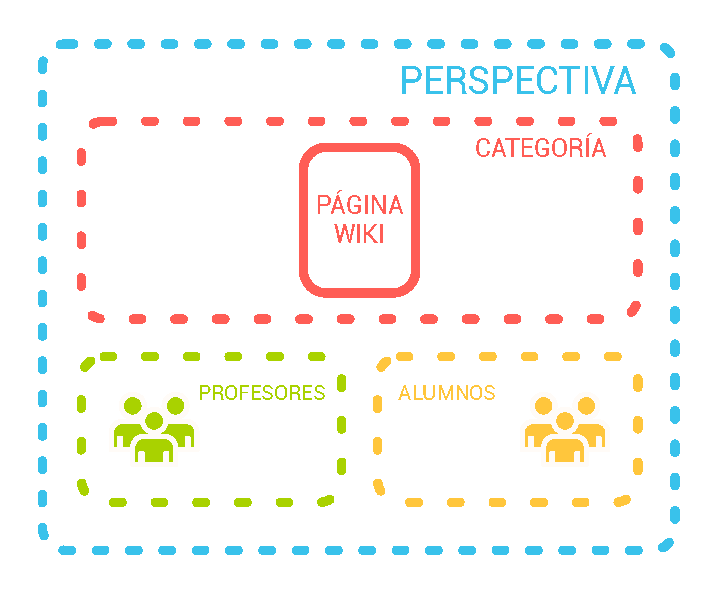
\includegraphics[width=.8\linewidth]{../graphics/fig_explicacion_profile_comunidad.eps}
\caption{Elementos que genera el \profile{} \texttt{Crear\_Comunidad\_de\_Practica\_Template}.}\label{fig:explicacion_profile_comunidad}
\end{figure}

\begin{itemize}
\item Se crea, por defecto, una página \textit{wiki} de bienvenida a la asignatura. Sirve como un punto de paso para cualquier miembro de la comunidad de práctica. Los posibles usos que se le pueden dar son variados, por ejemplo: se podría crear un listado de enlaces con las últimas novedades que han sucedido en la comunidad.

\begin{pyglist}[language=text]
  type: wiki_page
    ref: dashboard
    data:
     name: $profilerequest:nombre_asignatura$Asignatura sin nombre$ Homepage
     content: ”Bienvenido a tu nueva asignatura”
\end{pyglist}

\item Se crea una categoría que sirve para agrupar todos los elementos que se generen durante la actividad de la propia comunidad. Se utiliza por dos razones principalmente: la primera que así controlamos los permisos de dicha comunidad y sabemos, invariablemente, que sólo los miembros pueden actuar sobre los recursos que contiene; la segunda, los recursos quedan categorizados y facilitan la navegación y el orden dentro de \tiki{}.

\begin{pyglist}[language=text]
  objects: -
     type: category
     id: $project_root
     allow:
       - view
       - edit
       - wiki_view_history
       - wiki_view_source
       - minor
       - upload_picture
       - rollback
       - view_category
       - search
       - delete_account
       - group_view
       - group_view_members
       - add_object
       - modify_object_categories
\end{pyglist}

\item Se generan dos grupos: \textit{Profesores} y \textit{Alumnos} de dicha comunidad. Cada uno tienen unos permisos detallados, por ejemplo: los alumnos no pueden borrar las ediciones que hayan realizado en una página \textit{wiki} mientras que los profesores sí. Si un usuario no pertenece a ninguno de estos dos grupos (sea la comunidad de práctica que sea) se considera que no es miembro de ésta y por lo tanto no aparece la asignatura en el menú \textit{Asignaturas}.

\item Se crea una perspectiva que es la encargada de realizar el \q{cambio de contexto} de una comunidad de práctica a otra.

\begin{pyglist}[language=text]
  type: perspective
    ref: perspective
    data:
     name: $profilerequest:nombre_asignatura$sin nombre$
     preferences:
      category_jail: $project_root
      wikiHomePage: $dashboard
      browsertitle: $profilerequest:nombre_asignatura$Asignatura sin nombre$
      style: fivealive.css
      style_option: kiwi.css
      feature_wysiwyg: y
      wysiwyg_default: y
      wysiwyg_optional: y
\end{pyglist}

\item Por último se ajustan todos los permisos de manera adecuada por cada elemento creado anteriormente.

\begin{pyglist}[language=text]
  permissions:
   Member:
    autojoin: y
    allow:
        - view
        - edit
        - wiki_view_history
        - wiki_view_source
        - minor
        - upload_picture
        - rollback
        - view_category
        - search
\end{pyglist}
\end{itemize}

La implementación completa, tanto del \profile{} \texttt{Crear\_Comunidad\_de\_Practica\_Template} como del \texttt{Crear\_Comunidad\_de\_Practica\_GUI}, la podemos encontrar en la \sectionref{creacion-comunidad} y \sectionref{creacion-comunidad-gui}, respectivamente, del \appendixref{apendice-b}.